\section{Networking Theory}

\subsection{Raw Transmission of Bytes over Ethernet}

\subsubsection{Ethernet PHY Chip}
For transmission of raw data over ethernet a RMII 10/100 MHz ethernet transceiver (also called ethernet phy) is used, which is soldered onto the used development board and connected to the FPGA chip. Its model number is LAN8720A.

Its purpose is handling the low-level data handling and communication over ethernet, which includes
\begin{itemize}
  \item Decoding incoming data after receiving
  \item Encoding outgoing data before sending
  \item Negotiation of used speed or features with connection partner
\end{itemize}

More information about the LAN8720A can be found in its datasheet (\cite{smsc:lan8720a}).

\subsubsection{Reduced Media Independent Interface}
The Media Independent Interface (MII) and all its advanced versions like the used Reduced Media Independent Interface (RMII) are an established standard interface for connecting the Media Access Control (MAC) to an ethernet PHY. This ensures, that MACs need not to be modified, if another transmission medium with another PHY chip is required to be used.

The Medium Access Control is defined as any logic connected to a PHY over such a Media Independent Interface.

The signals defined in the specification for the RMII are listed in table \ref{table:rmii_signals}. REF\_CLK is the clock signal for data transmission and can be either a 50 MHz clock for 100 Mbit/s or a 5 MHz clock for 10 Mbit/s transmission speed. RXD is the data signal for incoming data. The PHY will set it, if it receives the next two bits of data. Data is valid, if CRS\_DV is asserted. If there has been an error while receiving the current two bits, RX\_ER is asserted. Outgoing data must be set at TXD two bits per clock cycle. The PHY will send those two bits out if TX\_EN is asserted. Transmissions of data of more than two bits are handled by consecutively handling all byte pairs of the message. \textbf{Important! TXD[0] is the first transmitted bit, RXD[0] is the first received bit.}

\begin{table}[]
  \centering
  \begin{tabular}{|c|c|c|c|}
    \hline
    \textbf{Signal name} & \textbf{\begin{tabular}[c]{@{}c@{}}Direction\\ (PHY)\end{tabular}} & \textbf{\begin{tabular}[c]{@{}c@{}}Direction\\ (MAC)\end{tabular}} & \textbf{Use} \\ \hline
    REF\_CLK & Input & \begin{tabular}[c]{@{}c@{}}Input or\\ Output\end{tabular} & \begin{tabular}[c]{@{}c@{}}Synchronous clock reference\\ for receive, transmit\\ and control interface\end{tabular} \\ \hline
    CRS\_DV & Output & Input & Carrier Sense/Receive Data Valid \\ \hline
    RXD{[}1:0{]} & Output & Input & Receive data \\ \hline
    TX\_EN & Input & Output & Transmit enable \\ \hline
    TXD{[}1:0{]} & Input & Output & Transmit data \\ \hline
    RX\_ER & Output & \begin{tabular}[c]{@{}c@{}}Input\\ (not required)\end{tabular} & Receive Error \\ \hline
  \end{tabular}
  \caption[Signals of the RMII specification]{Signals of the RMII specification. Taken from the official specification (\cite{rmii:spec}).}
  \label{table:rmii_signals}
\end{table}

\subsection{Transmission of Data via Protocol Packets}
The previous section explained, how raw data bits can be transmitted over ethernet connections utilizing an ethernet PHY chip and its reduced media independent interface. But in reality data is transmitted in packets and not in a raw form. These packets are called Ethernet packets or MAC packets and are part of the ethernet standardization IEEE 802.3. These packets enable different features such as error detection via checksums, sub-protocol multiplexing, routing and more. Information needed for these features is stored in headers of these packets and packets of sub-protocols can be stored within the data field of the parent protocols packet.

\subsubsection{Media Access Control Packets}
MAC packets are the lowest level packets. The structure of an ethernet packet is shown in figure~\ref{figure:mac_packet}. The fields of a MAC packet are:
\begin{itemize}
  \item \textbf{Preamble:} Sequence 10101010 10101010 10101010 10101010 10101010 10101010 10101010. \textbf{This sequence is transmitted from left to right.}
  \item \textbf{Start of Frame Delimiter (SFD):} Sequence 10101011. \textbf{This sequence is transmitted from left to right.}
  \item \textbf{Destination Address:} MAC address of packet recipient. \textbf{This address is transmitted least significant bit first octet-wise.}
  \item \textbf{Source Address:} MAC address of packet sender. \textbf{This address is transmitted least significant bit first octet-wise.}
  \item \textbf{Length / Type:} Number of octets in the mac client data (if value smaller or equal to 1500) or protocol used in mac client data (if value bigger or equal to 1536). For an embedded IP packet, the type value would be set as 0x0800. \textbf{This value is transmitted least significant bit first octet-wise.}
  \item \textbf{MAC Client Data:} Packet payload. Here are second level packets embedded. Must be between 46 and 1500 octets. If it is smaller than 46 octets, padding octets are added until the size is 46. \textbf{This value is transmitted least significant bit first octet-wise.}
  \item \textbf{Padding (PAD):} Padding octets included to ensure minimal packet length.
  \item \textbf{Frame Check Sequence (FCS):} CRC32 checksum of the packet. Calculated over the packet from MAC Destination Address through the payload. Calculation is described in section \ref{section:fcs}. \textbf{This value is transmitted most significant bit first, where the most significant bit is the coefficient belonging to the term \(x^{31}\) and the least significant bit is the coefficient belonging to the term \(x^0\).}
\end{itemize}

Between packets, there must be a transmission pause of 12 octets.

\begin{figure}[h]\label{figure:mac_packet}
  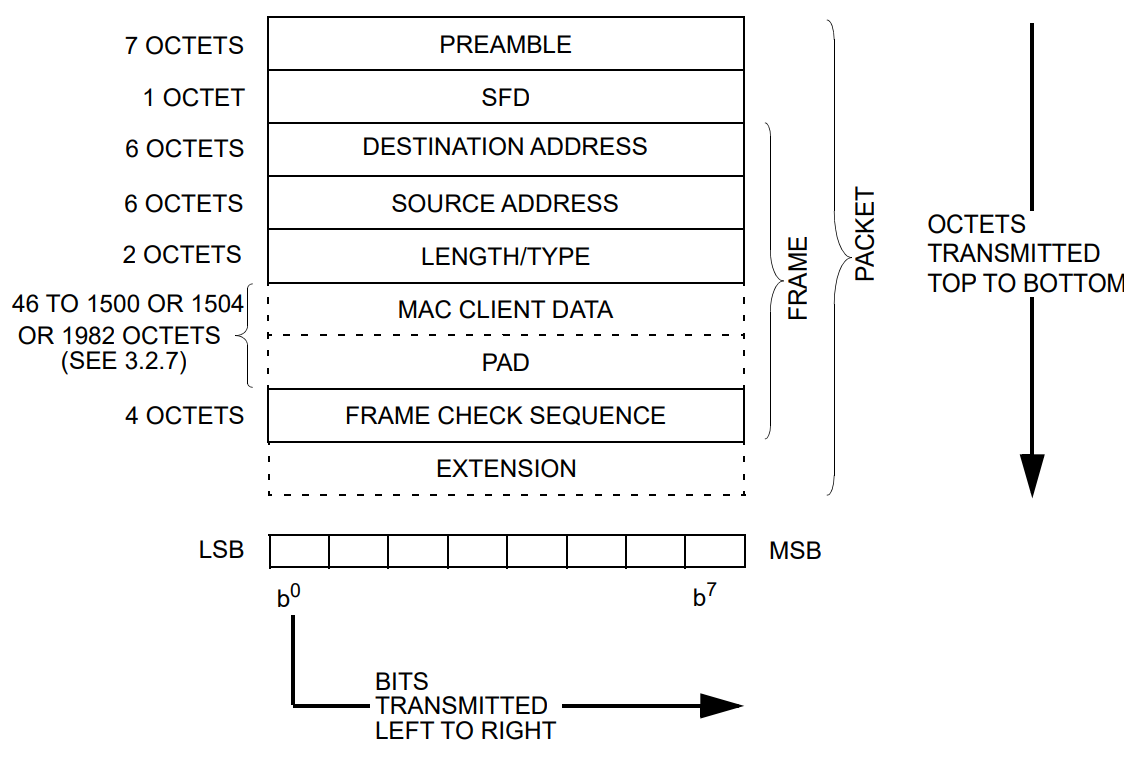
\includegraphics[width=\textwidth]{assets/mac_frame.png}
  \caption[Structure of an ethernet packet]{Structure of an ethernet packet. Field names are transmitted consecutively from top to bottom. TX\_EN is asserted while transmitting all fields except IPG.}
  \source{IEEE Standard for Ethernet~\cite{ieee:802.3}, page 119}
\end{figure}

% \begin{table}[]
%   \centering
%   \begin{tabular}{|c|c|c|}
%     \hline
%     \textbf{Field name} & \textbf{\begin{tabular}[c]{@{}c@{}}Size\\ (bits)\end{tabular}} & \textbf{Description} \\ \hline
%     Preamble & 56 & 7 bytes of 0xAA / 0b10101010 \\ \hline
%     Start of Frame Delimiter & 8 & 0xAB / 0b10101011 \\ \hline
%     MAC Destination Address & 48 & Packet destination address \\ \hline
%     MAC Source Address & 48 & Packet generator address \\ \hline
%     EtherType & 16 & Protocol of packet in payload \\ \hline
%     Payload & 46 - 1500 bytes & \begin{tabular}[c]{@{}c@{}}Packet payload data\\ (Includes higher level protocol\\ packets, e.g. IP packets)\end{tabular} \\ \hline
%     Frame Check Sequence & 32 & \begin{tabular}[c]{@{}c@{}}Packet checksum based\\ on CRC32 algorithm\end{tabular} \\ \hline
%     Interpacket gap (IPG) & 96 & \begin{tabular}[c]{@{}c@{}}Min. space between packets\\ (No Transmission)\end{tabular} \\ \hline
%   \end{tabular}
%   \caption[Structure of an ethernet packet]{Structure of an ethernet packet. Field names are transmitted consecutively from top to bottom. TX\_EN is asserted while transmitting all fields except IPG.}
%   \label{table:ethernet_packet}
% \end{table}

\subsubsection{IP Packets}
The IP protocol packet is a second level packet used for transmitting data over ethernet from one device to another utilizing 32 bit addresses. The structure of an IP packet is shown in table \ref{table:IP_packet}. The fields of an IP packet are:

% \begin{table}[]
%   \centering
%   \begin{tabular}{|c|c|c|}
%     \hline
%     \textbf{Field name} & \textbf{\begin{tabular}[c]{@{}c@{}}Size\\ (bits)\end{tabular}} & \textbf{Description} \\ \hline
%     Version & 4 & IP Version \\ \hline
%     IHL & 4 & Header length in 32 bit words \\ \hline
%     DSCP & 6 & Special additional options \\ \hline
%     ECN & 2 & Notification for network congestion \\ \hline
%     Total Length & 16 & Total length of IP packet \\ \hline
%     Identification & 16 & Unique ID \\ \hline
%     Flags & 3 & \begin{tabular}[c]{@{}c@{}}bit 0: reserved / always 0\\ bit 1: No Fragment\\ bit 2: More Fragments\end{tabular} \\ \hline
%     Fragment Offset & 13 & Offset of fragment in whole message \\ \hline
%     TTL & 8 & Time to live \\ \hline
%     Protocol & 8 & Protocol of packet in payload \\ \hline
%     Header Checksum & 16 & Checksum of header without payload \\ \hline
%     Source IP Address & 32 & Packet source address \\ \hline
%     Destination IP Address & 32 & Packet destination address \\ \hline
%     Options & 0 - 320 & Optional options - Used if IHL \textgreater~4 \\ \hline
%   \end{tabular}
%   \caption[Structure of an IP packet]{Structure of an IP packet. Field names are transmitted consecutively from top to bottom.}
  
% \end{table}

\newcolumntype{C}[1]{>{\centering\let\newline\\\arraybackslash\hspace{0pt}}m{#1}}

\begin{sidewaystable}
  \centering
  \begin{tabular}{|c*{32}{|@{}C{5mm}@{}}|}
  \hline
  \footnotesize{\textbf{Offset}} & \footnotesize{\textbf{0}} & \footnotesize{\textbf{1}} & \footnotesize{\textbf{2}} & \footnotesize{\textbf{3}} & \footnotesize{\textbf{4}} & \footnotesize{\textbf{5}} & \footnotesize{\textbf{6}} & \footnotesize{\textbf{7}} & \footnotesize{\textbf{8}} & \footnotesize{\textbf{9}} & \footnotesize{\textbf{10}} & \footnotesize{\textbf{11}} & \footnotesize{\textbf{12}} & \footnotesize{\textbf{13}} & \footnotesize{\textbf{14}} & \footnotesize{\textbf{15}} & \footnotesize{\textbf{16}} & \footnotesize{\textbf{17}} & \footnotesize{\textbf{18}} & \footnotesize{\textbf{19}} & \footnotesize{\textbf{20}} & \footnotesize{\textbf{21}} & \footnotesize{\textbf{22}} & \footnotesize{\textbf{23}} & \footnotesize{\textbf{24}} & \footnotesize{\textbf{25}} & \footnotesize{\textbf{26}} & \footnotesize{\textbf{27}} & \footnotesize{\textbf{28}} & \footnotesize{\textbf{29}} & \footnotesize{\textbf{30}} & \footnotesize{\textbf{31}} \\ 
  \hline
  0 & \multicolumn{4}{c|}{Version} & \multicolumn{4}{c|}{IHL} & \multicolumn{6}{c|}{DSCP} & \multicolumn{2}{@{}c@{}|}{ECN} & \multicolumn{16}{c|}{Total Length} \\ 
  \hline
  32 & \multicolumn{16}{c|}{Identification} & \multicolumn{3}{c|}{Flags} & \multicolumn{13}{c|}{Fragment Offset} \\ 
  \hline
  64 & \multicolumn{8}{c|}{Time to Live} & \multicolumn{8}{c|}{Protocol} & \multicolumn{16}{c|}{Header Checksum (optional)} \\ 
  \hline
  96 & \multicolumn{32}{c|}{Source IP Address} \\ 
  \hline
  128 & \multicolumn{32}{c|}{Destination IP Address} \\ 
  \hline
  160 & \multicolumn{32}{c|}{\multirow{3}{*}{Options (optional)}} \\ 
  \cline{1-1}
  ... & \multicolumn{32}{c|}{} \\ 
  \cline{1-1}
  448 & \multicolumn{32}{c|}{} \\
  \hline
  \end{tabular}
  \caption[Structure of an IP packet]{Structure of an IP packet. The first row and the leftmost column indicate the index of the bit.}
  \label{table:IP_packet}
\end{sidewaystable}

\begin{itemize}
  \item \textbf{Version:} The version of the IP protocol. Always 0x4 for IPv4.
  \item \textbf{IP Header Length (IHL):} Defines the length of the header in 32-bit words. A value of 0x5 means the normal header size of 20 bytes / 160 bits is used. Smaller values are not allowed. Bigger values enable optional options at the end of the header, which can be used for custom applications.
  \item \textbf{Differentiated Services Code Point (DSCP):} Very special options not needed for the vast majority of all IP applications.
  \item \textbf{Explicit Congestion Notification (ECN):} Same as DSCP.
  \item \textbf{Total Length:} Total length in bytes of an IP packet. It does not include inserted paddings of the ethernet packet for too small payloads.
  \item \textbf{Identification:} Unique identifier for packet. Used to assemble different fragments of the same packets.
  \item \textbf{Flag 1 / Reserved:} Always 0.
  \item \textbf{Flag 2 / Don't Fragment (DF):} If set, packet must not be fragmented.
  \item \textbf{Flag 3 / More Fragments (MF):} If set, there are more fragments of the packet. Not set on the last fragment.
  \item \textbf{Fragment Offset:} Offset to start of packet of the current fragment.
  \item \textbf{Time to Live (TTL):} Number of times the packet is passed along until it is dropped. This ensures, packets will not congest networks if stuck in a looped path.
  \item \textbf{Protocol:} Defines the used protocol of the packet within the payload. E.g. for UDP this value is 0x11.
  \item \textbf{Header Checksum:} This a simple checksum of the header values (excluding payload). This checksum is optional and can be left as value 0x0. Calculation of this checksum is explained in section \ref{section:basic_checksum}.
  \item \textbf{Source IP Address:} IP address of the packet sender.
  \item \textbf{Destination IP Address:} IP address of the packet recipient.
  \item \textbf{Options:} If IHL is bigger than 5, additional options are available. There are up to 20 additional bytes available, if IHL is set to its maximum value of 15. Those options are optional and can be used for custom purposes.
\end{itemize}

\subsubsection{UDP Packets}
The UDP protocol is a third level protocol used for transmitting data over ethernet from one device to another utilizing 16 bit ports. The structure of a UDP packet is shown in table \ref{table:UDP_packet}. The fields of an UDP packet are:

\begin{sidewaystable}
  \centering
  \begin{tabular}{|c*{32}{|@{}C{5mm}@{}}|}
  \hline
  \footnotesize{\textbf{Offset}} & \footnotesize{\textbf{0}} & \footnotesize{\textbf{1}} & \footnotesize{\textbf{2}} & \footnotesize{\textbf{3}} & \footnotesize{\textbf{4}} & \footnotesize{\textbf{5}} & \footnotesize{\textbf{6}} & \footnotesize{\textbf{7}} & \footnotesize{\textbf{8}} & \footnotesize{\textbf{9}} & \footnotesize{\textbf{10}} & \footnotesize{\textbf{11}} & \footnotesize{\textbf{12}} & \footnotesize{\textbf{13}} & \footnotesize{\textbf{14}} & \footnotesize{\textbf{15}} & \footnotesize{\textbf{16}} & \footnotesize{\textbf{17}} & \footnotesize{\textbf{18}} & \footnotesize{\textbf{19}} & \footnotesize{\textbf{20}} & \footnotesize{\textbf{21}} & \footnotesize{\textbf{22}} & \footnotesize{\textbf{23}} & \footnotesize{\textbf{24}} & \footnotesize{\textbf{25}} & \footnotesize{\textbf{26}} & \footnotesize{\textbf{27}} & \footnotesize{\textbf{28}} & \footnotesize{\textbf{29}} & \footnotesize{\textbf{30}} & \footnotesize{\textbf{31}} \\ 
  \hline
  0 & \multicolumn{32}{c|}{{\cellcolor[rgb]{0.753,0.753,0.753}}Source IP Address} \\ 
  \hline
  32 & \multicolumn{32}{c|}{{\cellcolor[rgb]{0.753,0.753,0.753}}Destination IP Address} \\ 
  \hline
  64 & \multicolumn{8}{c|}{{\cellcolor[rgb]{0.753,0.753,0.753}}0x00} & \multicolumn{8}{c|}{{\cellcolor[rgb]{0.753,0.753,0.753}}0x11} & \multicolumn{16}{c|}{{\cellcolor[rgb]{0.753,0.753,0.753}}Length} \\ 
  \hline
  96 & \multicolumn{16}{c|}{Source Port} & \multicolumn{16}{c|}{Destination Port} \\ 
  \hline
  128 & \multicolumn{16}{c|}{Length} & \multicolumn{16}{l|}{Checksum} \\
  \hline
  \end{tabular}
  \caption[Structure of a UDP packet]{Structure of a UDP packet. The first row and the leftmost column indicate the index of the bit. The grey rows indicate the UDP pseudoheader, which is included in the checksum, but not part of the real UDP header.}
  \label{table:UDP_packet}
\end{sidewaystable}

\begin{itemize}
  \item \textbf{Source Port:} The UDP port of the packet sender.
  \item \textbf{Destination Port:} The UDP port of the packet recipient.
  \item \textbf{Length:} The total length of the UDP packet. Like the length field of the IP packet header, it does not include inserted paddings of the ethernet packet for too small payloads.
  \item \textbf{Checksum:} The checksum of the UDP packet. This checksum is calculated over the whole UDP packet (header and payload) and the UDP packet pseudoheader. This pseudoheader consist of the IP source and destination addresses, the total UDP packet length and the value 0x0011. Unlike the one of IP packets is mandatory.
\end{itemize}

\subsection{Checksums}
Since checksums are an important tool to identify unwanted errors within a packet, most protocols make use of a checksum in its header. There are two kinds of checksums used in the networking context, which will be covered in depth in the following two sections.

\subsubsection{Standard Header Checksum}\label{section:basic_checksum}

\paragraph{What it is:}
This checksum is a 16-bit value. It is basically a one's complement addition of all byte pairs (16 bits) in a given packet and inverted result at the end.

\paragraph{Where it is used:}
This is the standard protocol header checksum. It is used in almost every protocol. In this project the IP and UDP protocols are used, which both utilize this checksum. But, in IP packets this checksum is optional.

\paragraph{How it is calculated:}
The checksum is calculated as follows:
\begin{enumerate}
  \item Split the whole message in byte pairs / 16 bits. If the message is not evenly divisible by 16 bits, append as many 0 bits as are needed to be divisible.
  \item Add two byte pairs of the message. If an overflow occurs, add it as well. Do this as long as there are byte pairs left in the message, which have not been added before.
  \item Invert the final result.
\end{enumerate}

\paragraph{How to verify message validity:}
After receiving a packet the checksum is calculated over the packet again. This time the packet includes the previously calculated checksum, so it is included in the second calculation. If the second calculation yields 0 as checksum, the packet has been transmitted without errors.

\paragraph{What else to consider:}
\begin{itemize}
  \item If the checksum has to be calculated of a packet, in which a checksum is normally included in the header, the checksum in the header will be set as 0.
  \item Addition of the overflow can also be delayed to the end for performance reasons. In this case all byte pairs should be summed into a 32 bit word. At the very end the upper 16 bytes and the lower 16 bytes should then be summed to yield the final sum.
\end{itemize}

\subsubsection{FCS / CRC32}\label{section:fcs}
In the realm of cyclic redundancy checks there exists a myriad of different implementations of cyclic redundancy check (CRC) with different bit sizes and additional special implementation details. Also, mathematically speaking, cyclic redundancy checks can be very complex and need a comprehensive study, which does not fit into the aim of this report. Therefore this sections only aims to describe the special implementation used in ethernet frames as frame check sequence (FCS) which is a type of cyclic redundancy check with 32 bits width (CRC32) and its special properties. For more in depth cover of the whole topic of cyclic redundancy check, the reader is encouraged to read a more detailed explanation of different kinds and implementations of cyclic redundancy checks in \cite{zlib.net:crc} or in the wikipedia articles about general cyclic redundancy checks in \cite{wikipedia.org:crc}, computation of cyclic redundancy checks in \cite{wikipedia.org:comp_crc} or mathematics of cyclic redundancy checks in \cite{wikipedia.org:math_crc}.

\paragraph{What it is:}
CRC32 stands for cyclic redundancy check with a polynomial of length 32 + 1. Cyclic redundancy check is a special kind of checksum based on polynomial arithmetic mod 2~\cite{wikipedia.org:crc} with a fixed predefined divisor polynomial.

\paragraph{Where it is used:}
This checksum is solely used as frame check sequence (FCS) attached to the back of the ethernet frame.

\paragraph{How it is calculated:}
The whole calculation is based on polynomial arithmetic mod 2 \cite{wikipedia.org:crc}, specifically on polynomial division. The whole packet is a series of bits which can be interpreted as a big polynomial, where each bit at index $i$ in the message corresponds to the coefficient of the term \(x^{L - i}\) with the message length $L$. This polynomial is then divided by a predefined divisor, which is defined as 0x104C11DB7 in the ethernet context. This value corresponds to the polynomial
\begin{equation}
  x^{32} + x^{26} + x^{23} + x^{22} + x^{16} + x^{12} + x^{11} + x^{10} + x^{8} + x^{7} + x^{5} + x^{4} + x^{2} + x + 1.
\end{equation}
Every bit in the value denotes the coefficient of the term x to the power of the bit index. An example illustrating polynomial division is shown in \ref{polynomial_division}. For more comprehensive examples and descriptions see \cite{wikipedia.org:crc} or \cite{zlib.net:crc}.

The frame check sequence is a slightly modified version of this polynomial division. The single steps for calculating the frame check sequence are the following:
\begin{enumerate}
  \item Append 32 binary zeroes to the message.
  \item Invert the first 32 bits of the message.
  \item Do polynomial division of the message with the divisor 0x104C11DB7 until a rest remains, like shown in the steps above.
  \item The rest is a 32 bits long word. Invert it to get the checksum.
\end{enumerate}

\paragraph{How to verify message validity:}
After receiving a packet the frame check sequence is calculated over the whole ethernet frame including the frame check sequence again. If the calculated frame check sequence matches the magic number 0x38fb2284, then the frame has been transmitted without errors.

\paragraph{What else to consider:}
\begin{itemize}
  \item Since data bytes are transmitted least significant bit first over ethernet, every byte must be reversed after receiving and before CRC32 calculation.
  \item The above mentioned approach to calculating the frame check sequence has two major drawbacks in hardware implementations. Firstly, every clock cycle only one bit can be handled and secondly at the end there must be 32 bits added. Therefore different approaches have been developed providing a possibility to calculate the fcs with more bits at once fed into
  
  FCS calculation usually requires adding 32 binary zeroes to the message. This can result in poor performance in hardware, if the checksum is calculated continuously while receiving data. Therefore, in this project another solution has been used, which does not require adding zeroes and can be calculated with only binary logic operations. The logic behind it is described in 
\end{itemize}
